\begin{frame}{照射されたKaonの数 {\bf (Run68) }}
  \label{page:Knum}
  
  \footnotesize
  \tminipageTwo{
    \begin{figure}
      相対比率\\
      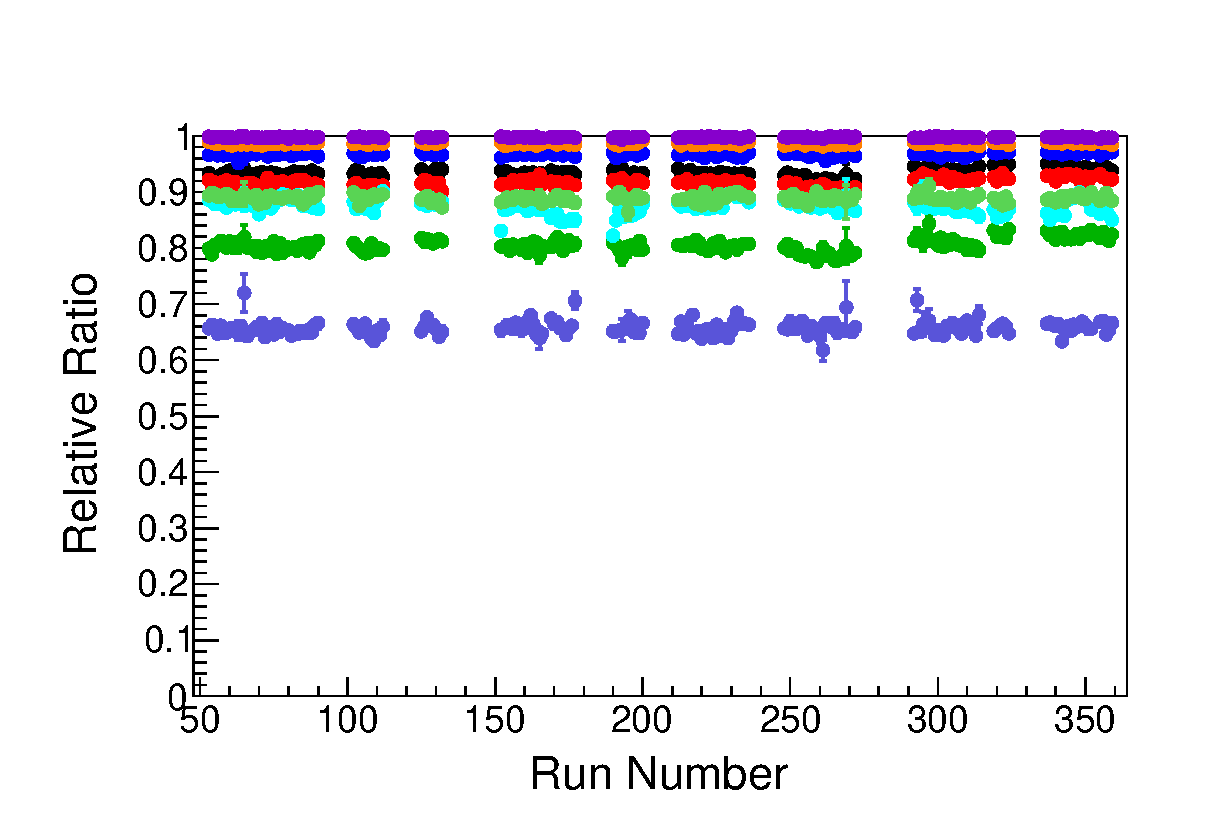
\includegraphics[width=4cm]{../pic/Run68/BL/relative_ratio.eps}
    \end{figure}
    \centering
    \vspace{-4mm}
    \scriptsize
    前の条件に対する有効なイベントの比率
  }{
    \begin{figure}
      生き残り率\\
      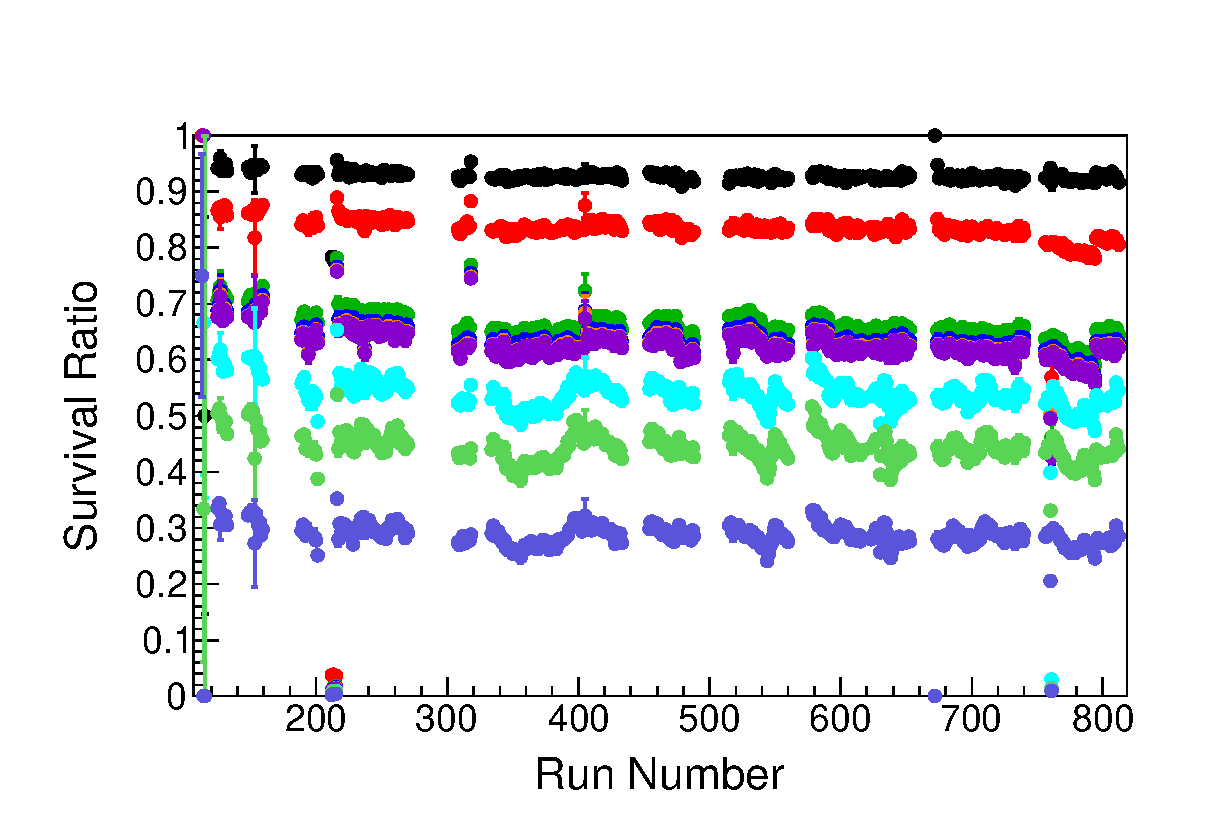
\includegraphics[width=4cm]{../pic/Run68/BL/survival_ratio.eps}
    \end{figure}
    \centering
    \vspace{-4mm}
    \scriptsize
    最初の条件に対する有効なイベントの比率
  }


  \tminipageTwo{
    照射されたKaonの数はスケーラーの値を\\
    Kaonビームとして解析できた比率で計算する\\
    %% { \tiny
    %%   p.\pageref{page:BL_item}参照
    %% }
  }{
    \begin{figure}
      照射されたKaonの数
      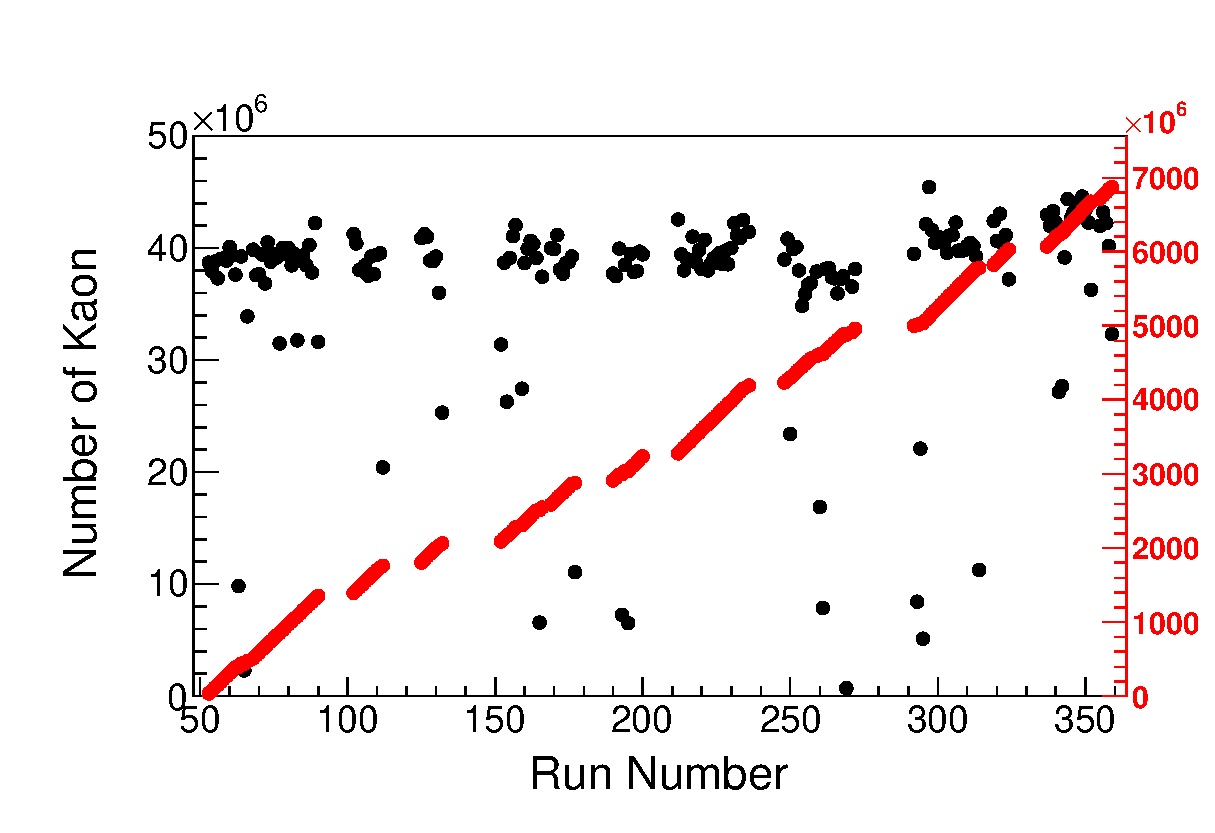
\includegraphics[width=4cm]{../pic/Run68/BL/Knum.eps}
    \end{figure}
    \centering
    \vspace{-4mm}
    \scriptsize
    黒は各ランの照射された数\\
    赤は照射された数の総和
  }
\end{frame}
